\documentclass[handout]{beamer}
%\documentclass{beamer}
\usepackage{tikz}
\def\checkmark{\tikz\fill[scale=0.4](0,.35) -- (.25,0) -- (1,.7) -- (.25,.15) -- cycle;} 
\usepackage{pifont}
\newcommand{\xmark}{\ding{55}}
\usepackage{tikz}
\usepackage{biblatex}
\usetheme{PaloAlto}
\title{An introduction to Bayesian inference}
\author[Ben Lambert]{Ben Lambert\inst{1}\\ \texttt{ben.c.lambert@gmail.com}}
\usepackage{datetime}
\date{}
\institute[University of Oxford]{
\inst{1}University of Oxford}
\beamertemplatenavigationsymbolsempty
\setbeamertemplate{sidebar left}{}
\usepackage{caption}
\usepackage{amsmath}
\usepackage{soul,xcolor}
\usepackage{multimedia}
\usepackage{animate}
\usepackage{graphics}
\usepackage{graphicx}
\usepackage[makeroom]{cancel}
\usepackage{xcolor,cancel}
\captionsetup{font=footnotesize}
\usepackage[utf8]{inputenc}
\makeatletter
\newcommand\mathcircled[1]{%
  \mathpalette\@mathcircled{#1}%
}
\newcommand\@mathcircled[2]{%
  \tikz[baseline=(math.base)] \node[draw,circle,inner sep=1pt] (math) {$\m@th#1#2$};%
}
\makeatother
\definecolor{beige}{RGB}{238,213,173}

\newcommand\hcancel[2][black]{\setbox0=\hbox{$#2$}%
	\rlap{\raisebox{.45\ht0}{\textcolor{#1}{\rule{\wd0}{1pt}}}}#2} 

\bibliography{Bayes}

\begin{document}

\begin{frame}
\titlepage
\end{frame}

\begin{frame}
	\frametitle{Who am I?}
	\begin{itemize}
		\item Statistician working on data science, machine learning and statistical inference across the university.
		\item User of Bayesian statistics for the past X years.
		\item Born in the same town as Thomas Bayes (Tunbridge Wells).
	\end{itemize}
	
	\onslide<1->
	\begin{figure}[ht]
		\centerline{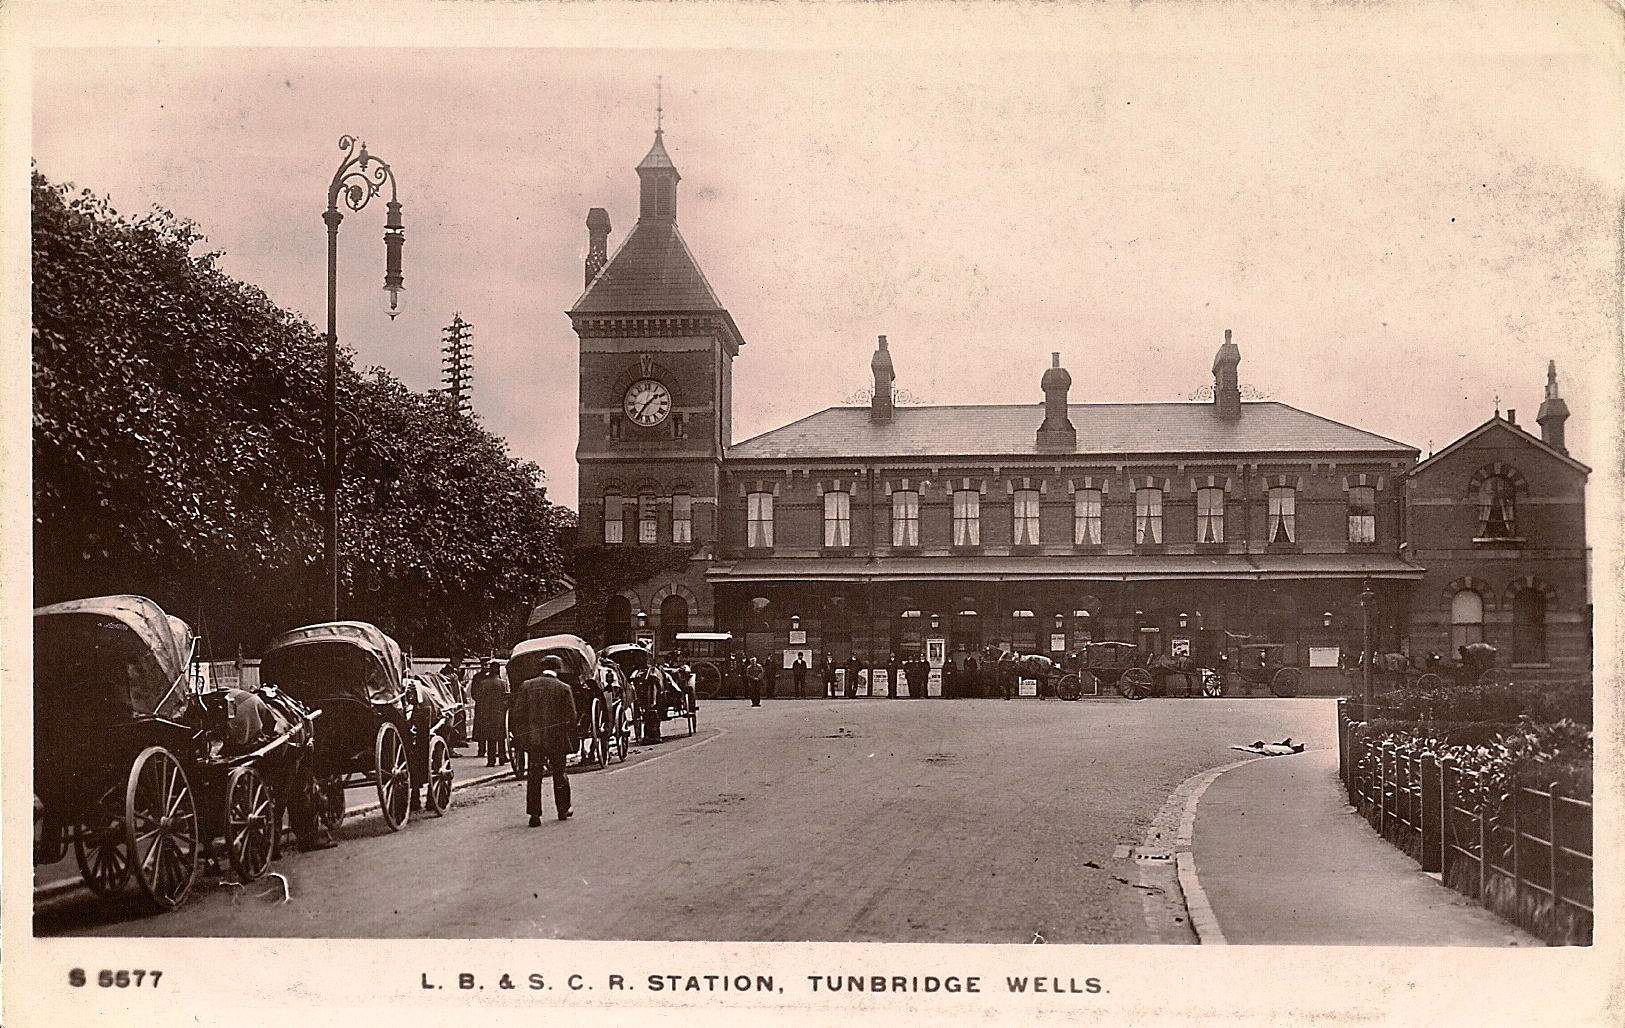
\includegraphics[width=0.6\textwidth]{./animations_figures/tunbridgeWells.jpg}}
	\end{figure}
	
\end{frame}

\begin{frame}
	\frametitle{Course timetable}
	
	Today:
	
	\begin{itemize}
		\item<2-> Lecture from 9.30am - 10.30am: an introduction to Bayesian inference.
		\item<3-> Problem class from 10:40am - 12:30pm.
		\item<4-> Lecture from 2pm - 2:30pm: A romp through MCMC and short ABC introduction.
		\item<5-> Problem class from 3pm - 5pm.
	\end{itemize}
	
	Lecture notes on Canvas.
	
\end{frame}


\begin{frame}
	\frametitle{Lecture outcomes}
	By the end of this lecture you should:
	
	\begin{itemize}
		\item Know what probability distributions are and why they are used in modelling.
		\item Understand the goal of statistical inference.
		\item Appreciate how Bayesian and frequentist approaches to inference achieve this goal.
		\item Know the elements required to do Bayesian inference and appreciate how they affect inferences.
		\item Know why exact Bayesian inference is \textit{hard}.
		\item See how conjugate priors provide a slight remedy.
	\end{itemize}
	
\end{frame}

\begin{frame}
	\frametitle{Why don't more people use Bayesian inference?}
	
	\begin{itemize}
		\item<2-> Most existing texts put a strong emphasis on its (seemingly) complex mathematical basis.
		\item<3-> Poor explanation of why computational sampling (usually MCMC) is needed.
		\item<5-> The view that Bayesian inference is more wishy-washy than frequentist inference. 
	\end{itemize}
\end{frame}

\begin{frame}
	\frametitle{Tangible benefits of Bayesian inference}
	
	\begin{itemize}
		\item<2-> Simple and intuitive model building (unlike frequentist statistics there is no need to remember lots of specific formulae).
		\item<3-> Exhaustive and creative model testing.
		\item<4-> The best predictions; for example, Nate Silver.
		\item<5-> Allows estimation of models that would be impossible in frequentist statistics: especially true in epidemiology!
	\end{itemize}
	
	\onslide<5->
	\begin{figure}[ht]
		\centerline{
\includegraphics[width=0.3\textwidth]{./animations_figures/nateSilver.jpg}}
	\end{figure}
	
\end{frame}

\begin{frame}
	\frametitle{Books I recommend}
	
	\onslide<1->
	\begin{figure}[ht]
		\centerline{\includegraphics[width=1\textwidth]{./animations_figures/bayesbooks.pdf}}
	\end{figure}
\end{frame}

\begin{frame}
	\frametitle{Outline}
	\tableofcontents
\end{frame}

\section{An introduction to statistical modelling}
\frame{\tableofcontents[currentsection]}

\begin{frame}
	\frametitle{Example: how to estimate disease prevalence?}
	
	\begin{itemize}
		\item Suppose we take a sample of $N$ study participants from the population.
		\item We take their blood and use a clinical test to determine presence / absence of disease: finding $X$ are disease-positive.
	\end{itemize}
	
	Question: How do we use these data to estimate disease prevalence (with uncertainty)?
	
\end{frame}

\begin{frame}
	\frametitle{Building a model to explain these data}
	
	We don't know a lot about how our data were produced:
	
	\begin{itemize}
	\item How exactly participants were picked.
	\item How the disease is distributed in the population.
	\item How the clinical test works.
	\end{itemize}
	
	Due to uncertainty $\implies$ use a model that encompasses uncertainty: i.e. one that uses probability distributions.
	
\end{frame}

\begin{frame}
	\frametitle{Which probability distribution?}
	
		\begin{figure}[h]
			\centerline{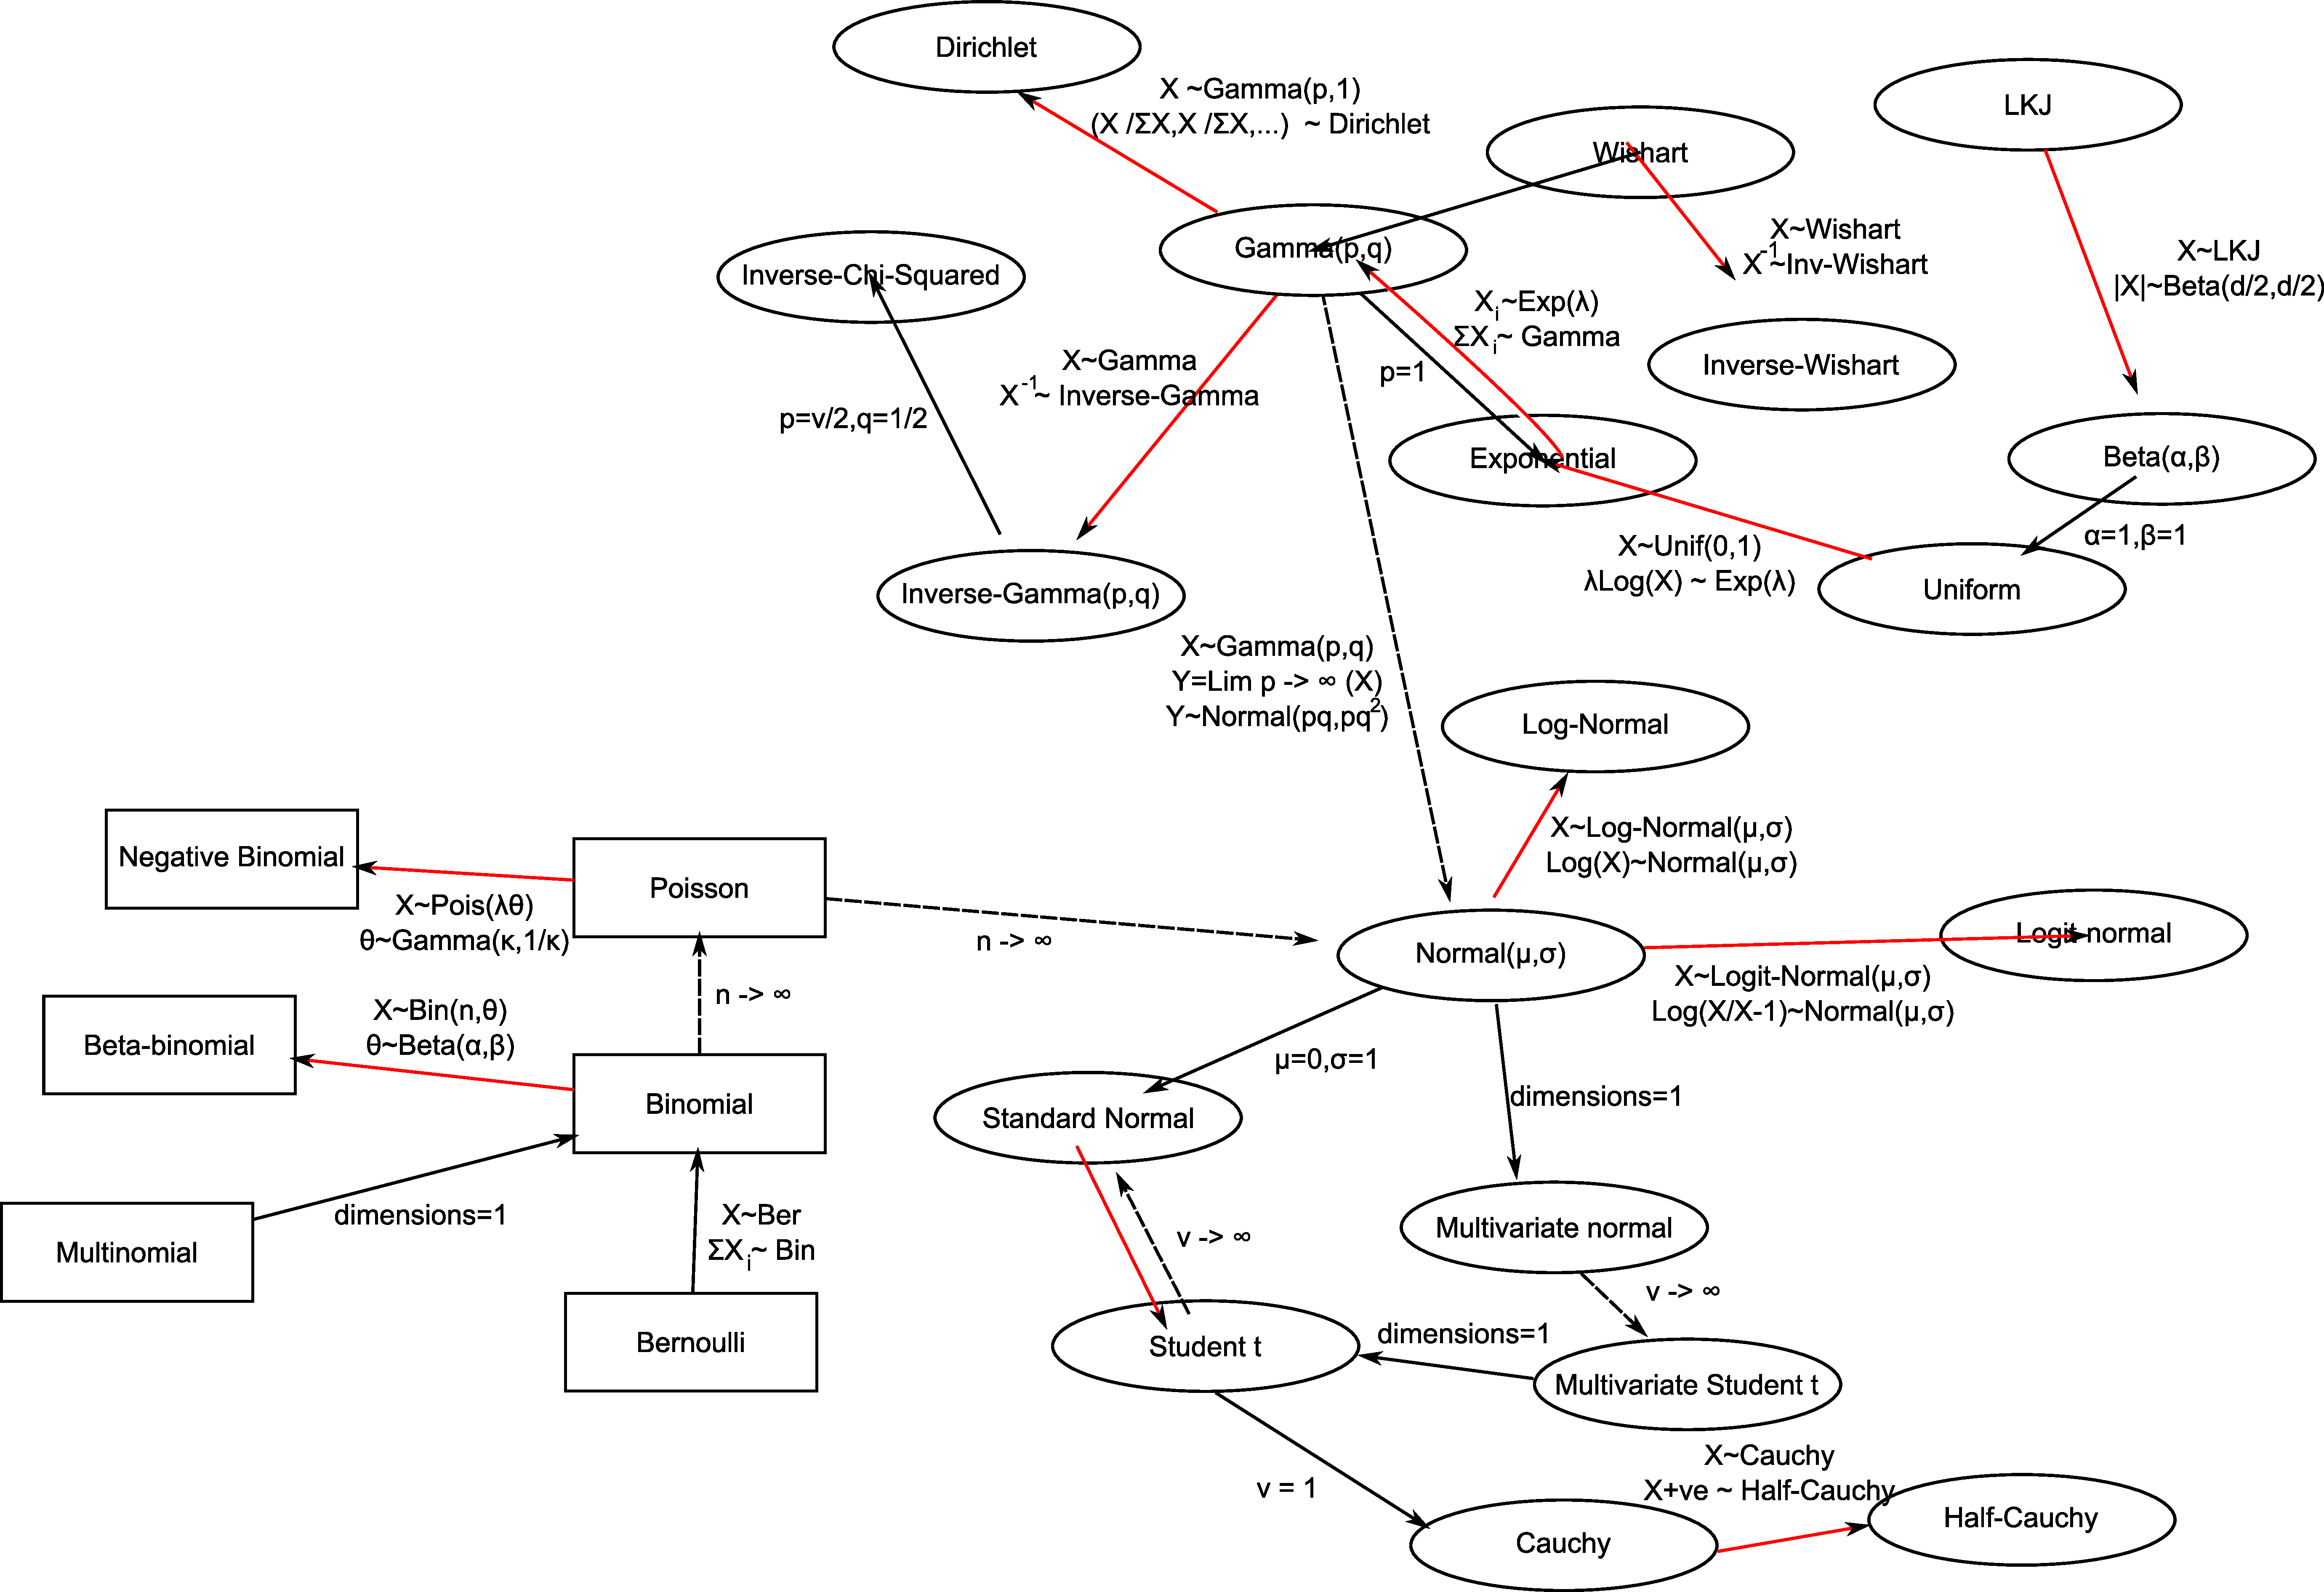
\includegraphics[width=1\textwidth]{animations_figures/Distributions_nexusOfRelations.pdf}}
		\end{figure}
	
\end{frame}


\begin{frame}
	\frametitle{How to choose a probability model?}
	
	Characteristics of our data:
	
	\begin{enumerate}
		\item Our sample size $N$ is fixed.
		\item Our data $X$ are discrete and can take values $0, 1, 2, ..., N-1, N$.
	\end{enumerate}
	
	Assumptions:
	
	\begin{enumerate}
		\item Individuals represent independent samples from a population.
		\item Those individuals are drawn from the same population.
	\end{enumerate}
	
\end{frame}

\begin{frame}
	\frametitle{Which probability model satisfies these conditions?}
	\begin{figure}[h]
		\centerline{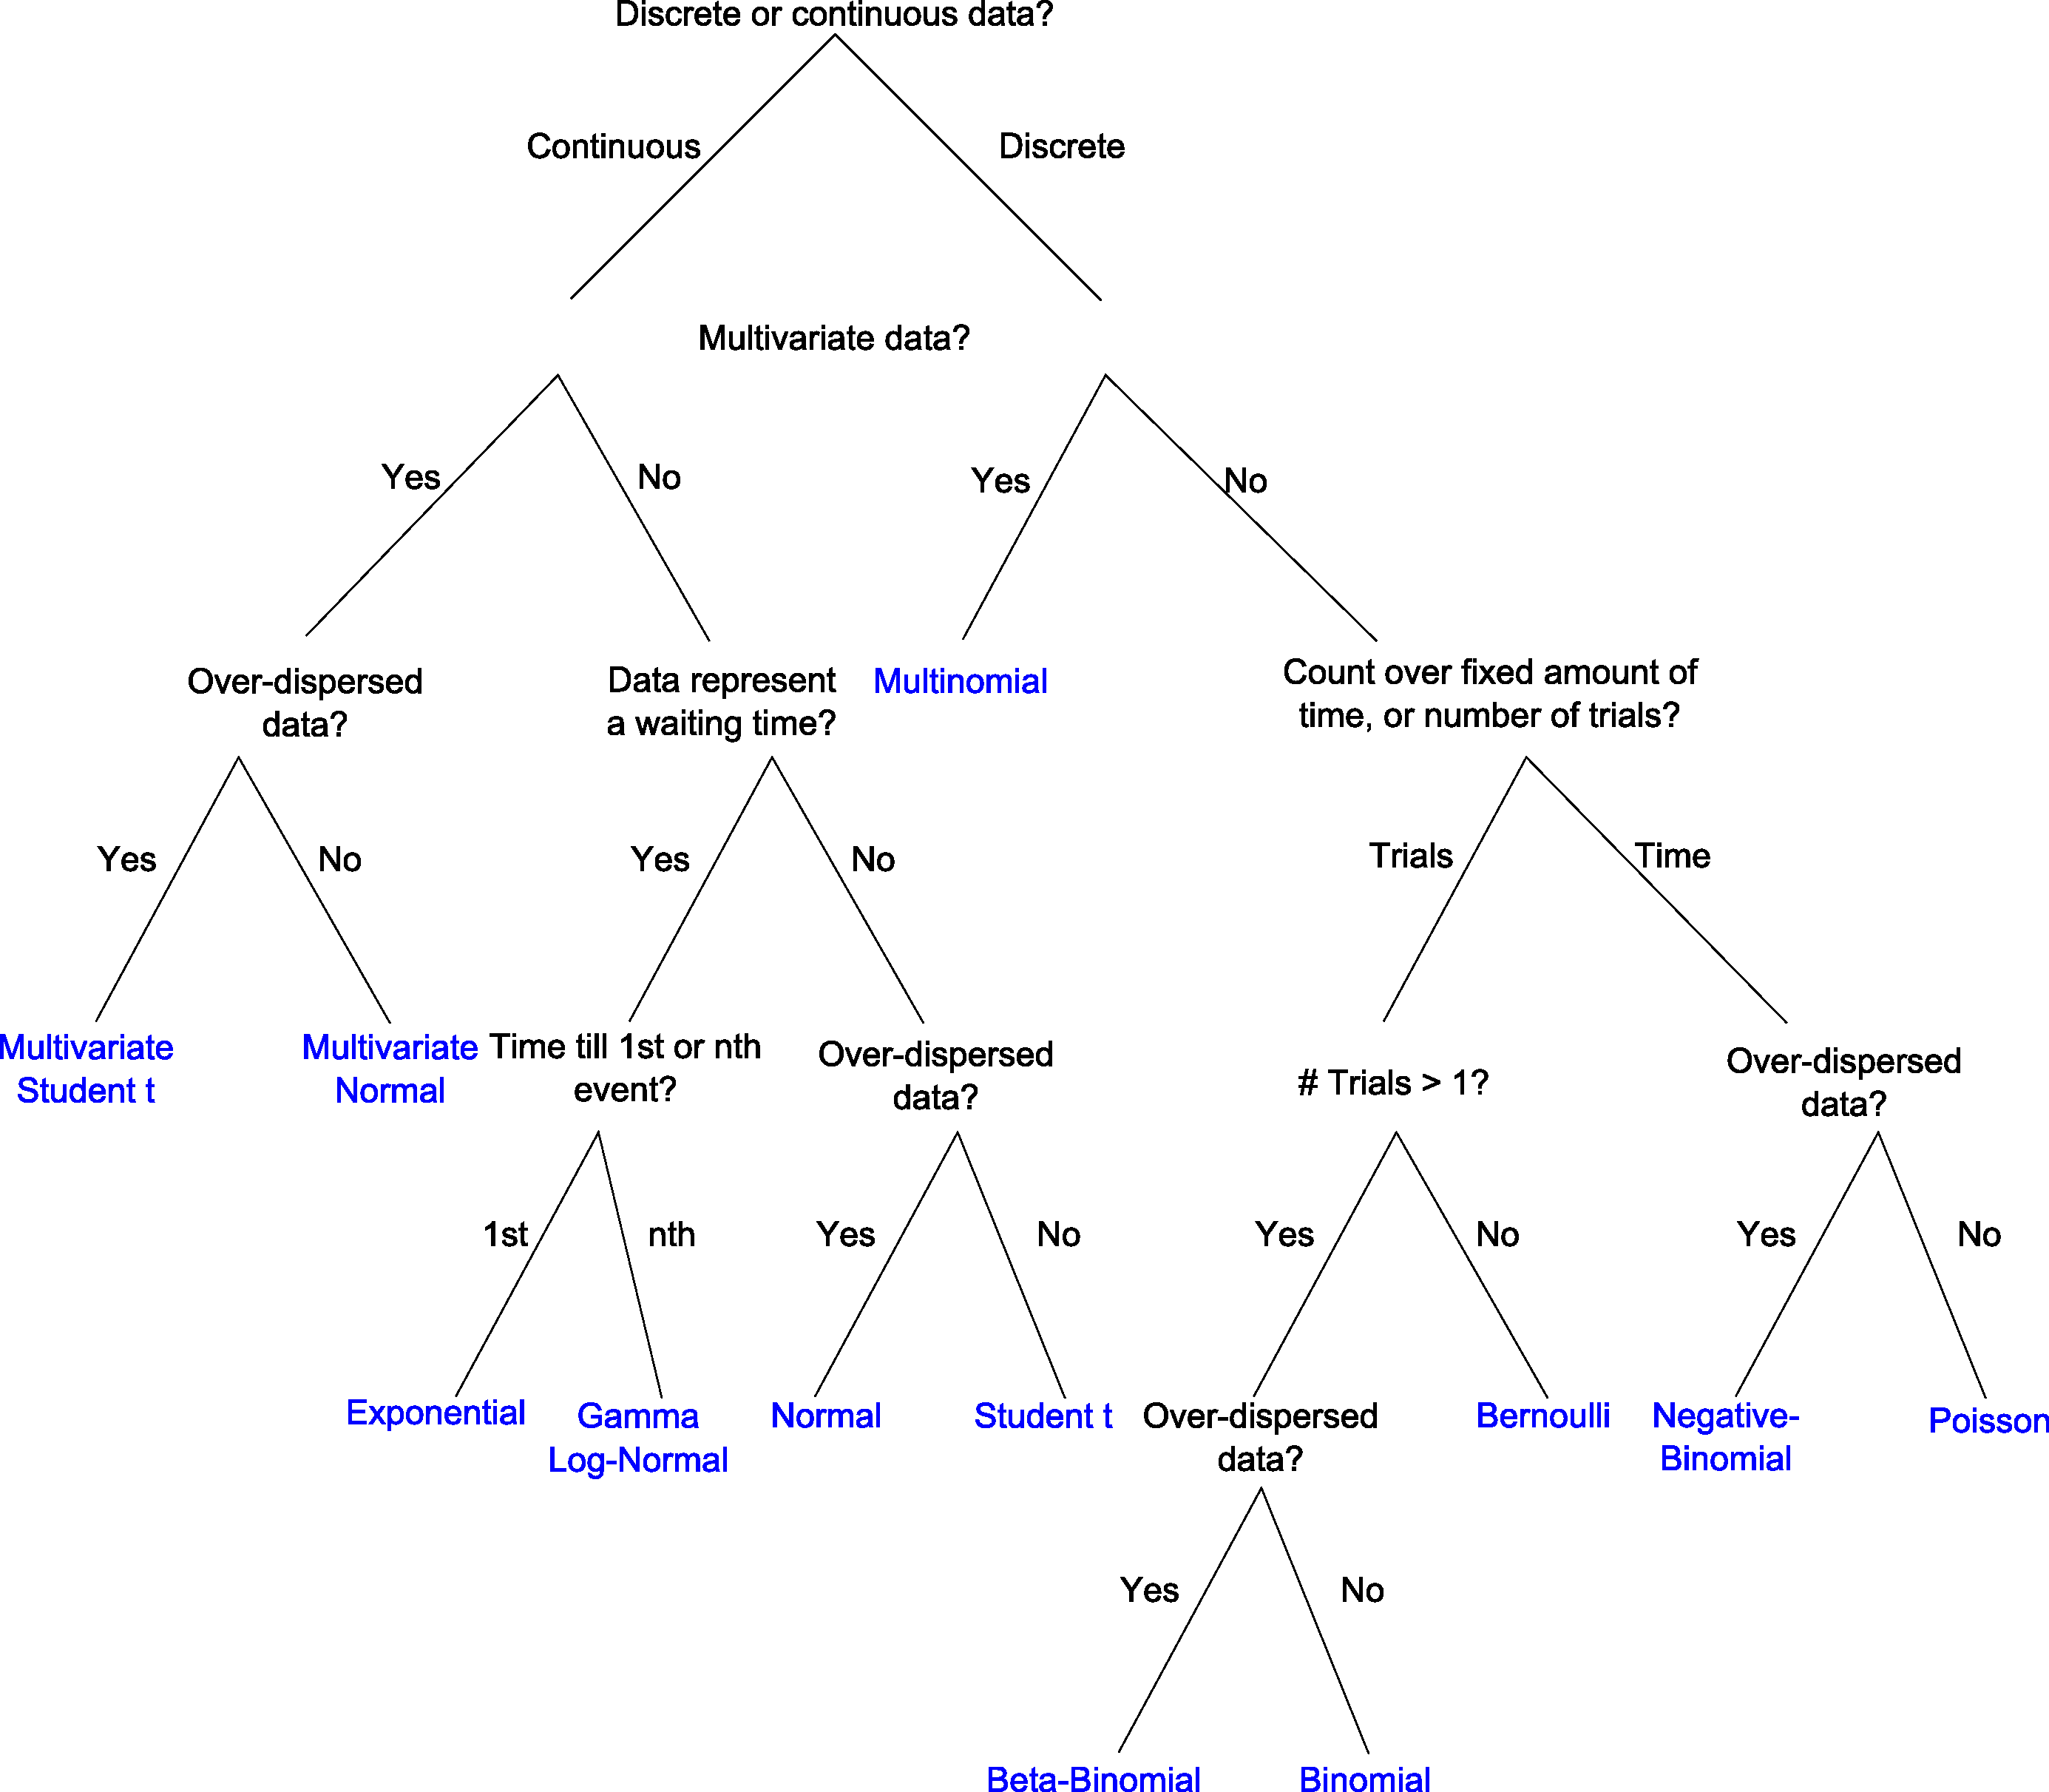
\includegraphics[width=0.8\textwidth]{animations_figures/Distributions_likelihoodTree.pdf}}
	\end{figure}
	
\end{frame}

\begin{frame}
	\frametitle{Binomial model: introduction}
	
	Analogy: count of disease-positive cases in a sample of size $N$ $\sim$ count of a coin landing heads up in $N$ flips of it.
	
	\vspace{0.2cm}
	
	If we assume the clinical test is perfect:
	
	\begin{itemize}
		\item $\text{Pr}(+) = \theta$ is the proportion of disease-positive individuals in the population.
		\item Analogous to $\text{Pr}(H) = \theta$, the probability the coin lands heads up: $0\leq \theta \leq 1$.
	\end{itemize}
	
\end{frame}

\begin{frame}
	\frametitle{Binomial model probability}
	The probability of a given number of heads $X$ depends on:
	
	\begin{itemize}
		\item $\text{Pr}(H) = \theta$.
		\item The number of possible ways to obtain result. E.g. if $N=2$, there are two ways to obtain $X=1$: $(1,0)$ or $(0,1)$.
		\end{itemize}
\end{frame}

\begin{frame}
	\frametitle{Binomial model probability}
	The probability for a given $X$ is:
	
	\begin{equation}
	\text{Pr}(X|\theta) = \binom{N}{X} \theta^X (1- \theta)^{N-X}.
	\end{equation}
	
	We often use the following notation as shorthand:
	
	\begin{equation}
	X\sim \mathcal{B}(N, \theta).
	\end{equation}
	
\end{frame}

\begin{frame}
	\frametitle{Binomial model probabilities: visualised}
	
	Suppose $\theta=0.5$ and $N=10$.
	
	\begin{figure}[h]
		\centerline{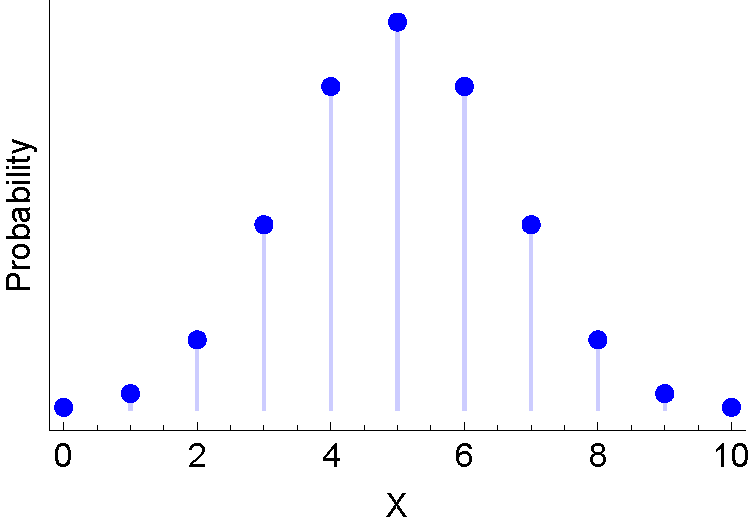
\includegraphics[width=0.8\textwidth]{animations_figures/binomial.pdf}}
	\end{figure}
	
\end{frame}

\section{The goal of statistical inference}
\frame{\tableofcontents[currentsection]}


\begin{frame}
	\frametitle{Many ways of generating data}
	
	Suppose:
	
	\begin{itemize}
		\item We take blood from $N=10$ patients.
		\item And find that $X=3$ individuals are disease-positive.
	\end{itemize}
	
	How could this have happened?
	
\end{frame}

\begin{frame}
	\frametitle{Many worlds are consistent with data}
	
	\begin{figure}[h]
		\centerline{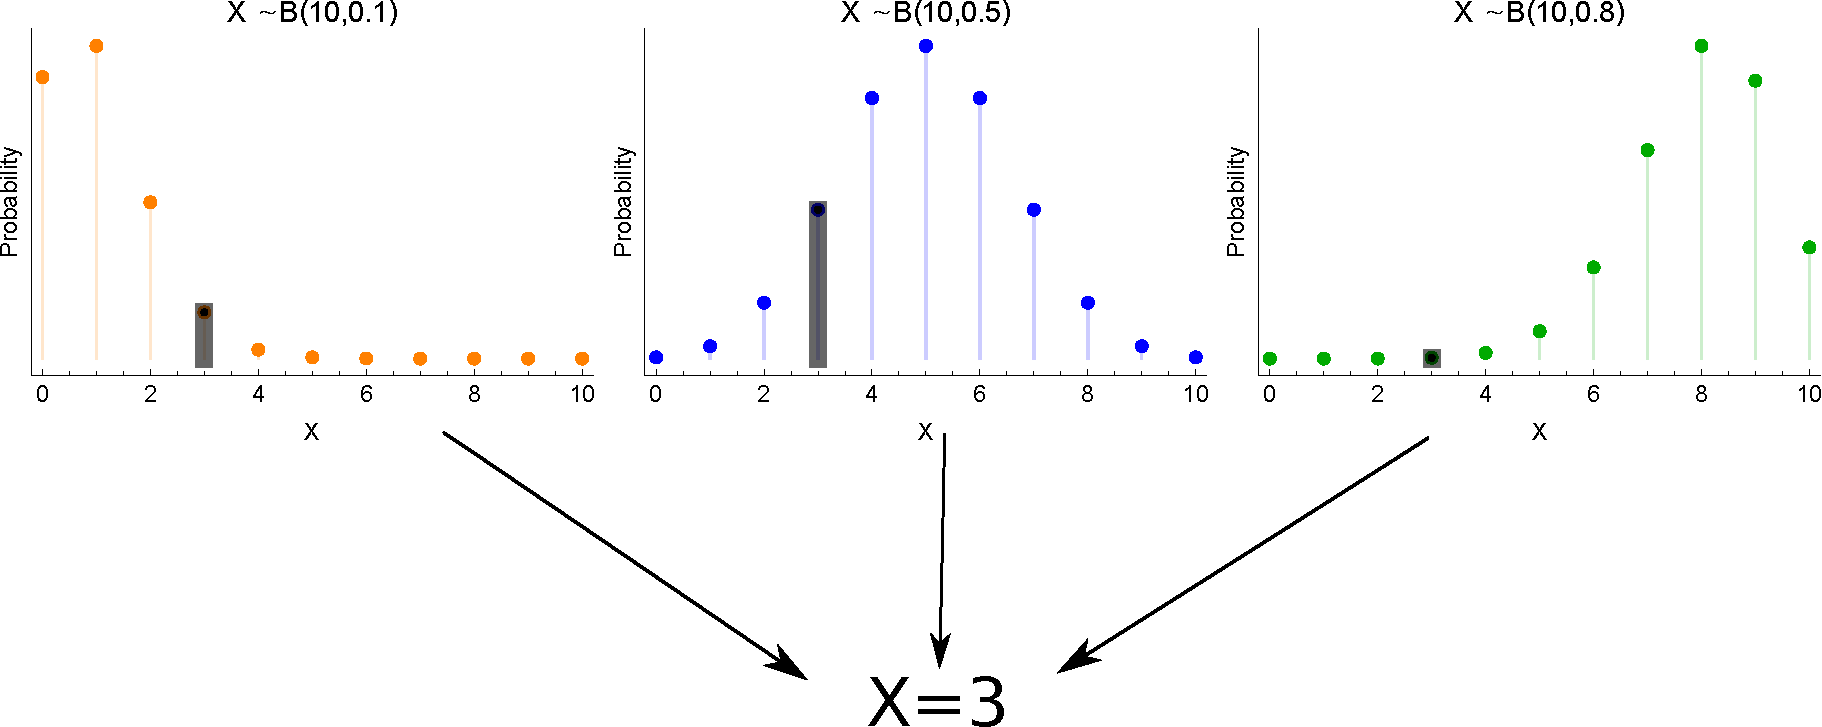
\includegraphics[width=1\textwidth]{animations_figures/binomial_many_worlds_inkscaped.pdf}}
	\end{figure}
	
\end{frame}

\begin{frame}
	\frametitle{Aim of inference: determine which worlds are most likely}
	\begin{figure}[h]
		\centerline{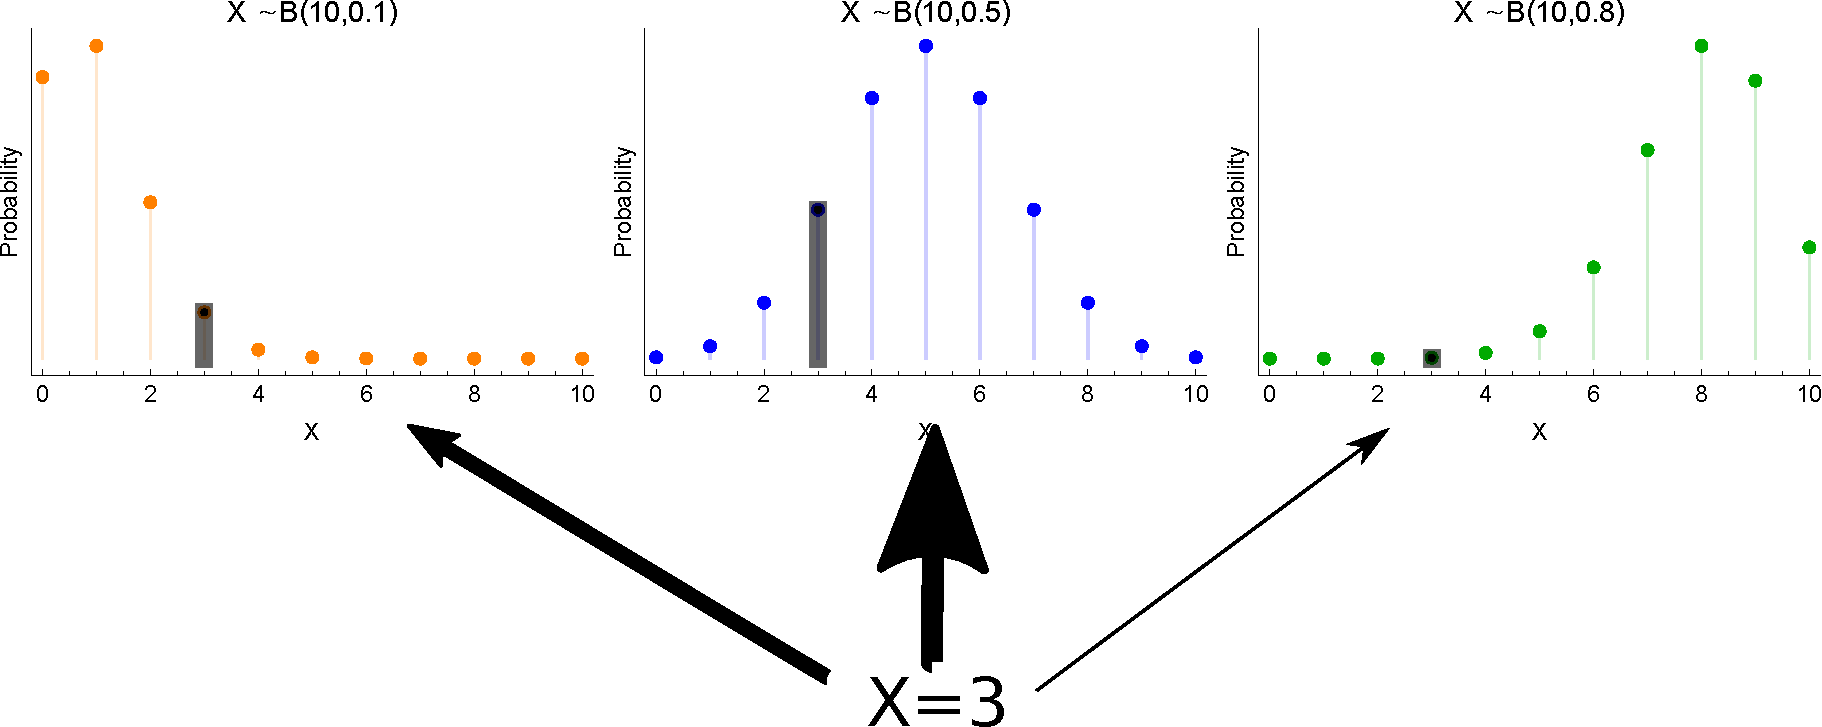
\includegraphics[width=1\textwidth]{animations_figures/binomial_many_worlds_inverse.pdf}}
	\end{figure}
\end{frame}

\begin{frame}
	\frametitle{Inference is effectively inverting our model}
	
	\begin{itemize}
		\item Forward model: our probability model $X\sim \mathcal{B}(10,\theta)$ gives us an (infinite) number of ways to \textit{generate} data: one for each value of $\theta$.
		\item Inverse model: in inference, instead start with $X$ and want to run process in reverse to determine which values of $\theta$ could have generated it.
	\end{itemize}
	
	Inference amounts to going from an effect -- the data -- back to its cause -- the parameter values.
	
\end{frame}

\begin{frame}
	\frametitle{Likelihoods versus probability distributions}
	
	The binomial probability model:
	
	\begin{equation}
	\text{Pr}(X|\theta) = \binom{N}{X} \theta^X (1- \theta)^{N-X}.
	\end{equation}
	
	can be used to calculate the probability of different values of $X$ for a fixed $\theta$. This amounts to using the \textit{forward} or \textit{generative} model.
	
\end{frame}

\begin{frame}
	\frametitle{A probability distribution}
	For $\theta=0.5$, we can calculate probabilities:
	
	\begin{figure}[h]
		\centerline{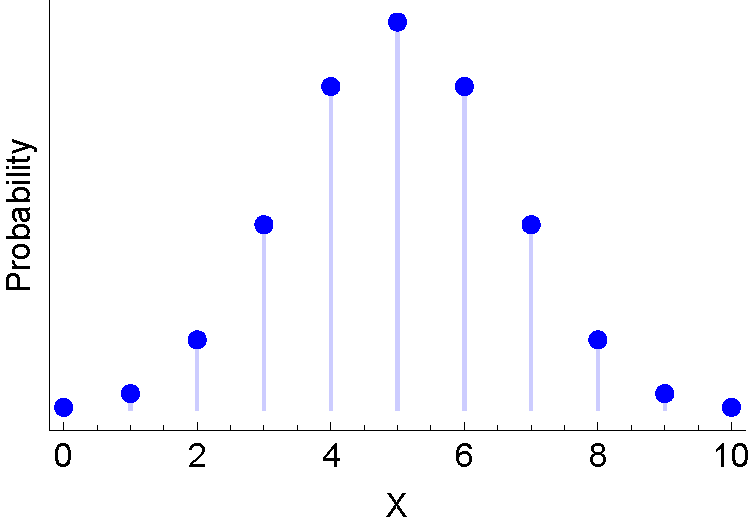
\includegraphics[width=0.8\textwidth]{animations_figures/binomial.pdf}}
	\end{figure}

\end{frame}

\begin{frame}
	\frametitle{Likelihoods versus probability distributions}
	In inference, we have fixed $X=3$ -- our observed data. Now we can vary $\theta$ and use:
	
		\begin{equation}
		\text{Pr}(X|\theta) = \binom{N}{X} \theta^X (1- \theta)^{N-X} = 120 \theta^3 (1-\theta)^7
		\end{equation}
		
	to calculate what are known as likelihoods of each value of $\theta$.
	
\end{frame}

\begin{frame}
	\frametitle{Likelihood function}
	
	\begin{figure}[h]
		\centerline{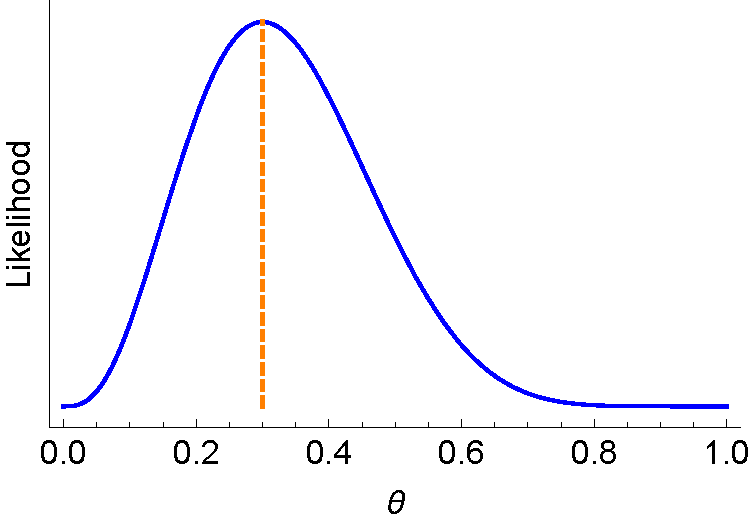
\includegraphics[width=1\textwidth]{animations_figures/binomial_likelihood_eg.pdf}}
	\end{figure}
	
\end{frame}

\begin{frame}
	\frametitle{Why is a likelihood function not a valid probability distribution?}
	
	\begin{figure}[h]
		\centerline{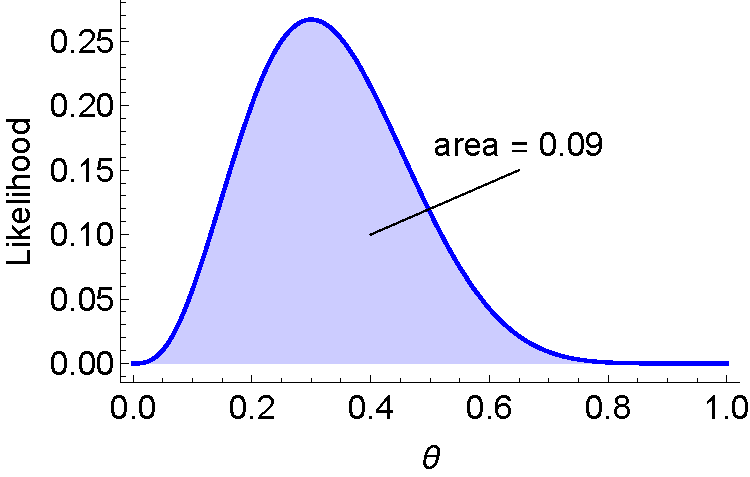
\includegraphics[width=1\textwidth]{animations_figures/binomial_likelihood_area.pdf}}
	\end{figure}
	
\end{frame}

\begin{frame}
	\frametitle{}
	{\Huge Questions?}
\end{frame}

\section{Frequentist and Bayesian world views}
\frame{\tableofcontents[currentsection]}

\begin{frame}
	\frametitle{Why do we care about likelihoods?}
	Two predominant approaches to inference:
	
	\begin{itemize}
		\item Frequentist inference.
		\item Bayesian inference.
	\end{itemize}
	
	Both use likelihoods as a basis of inference.
	
\end{frame}

\begin{frame}
	\frametitle{The aim of inference: inverting the likelihood}
	
	\begin{itemize}
		\item Both frequentists and Bayesians essentially invert: $p(X|\theta)\rightarrow p(\theta|X)$.
		\item Both attempts to convert the likelihood into a probability distribution.
		\item Their methods of inversion are \textit{different}.
	\end{itemize}
	
	\begin{figure}[ht]
		\centerline{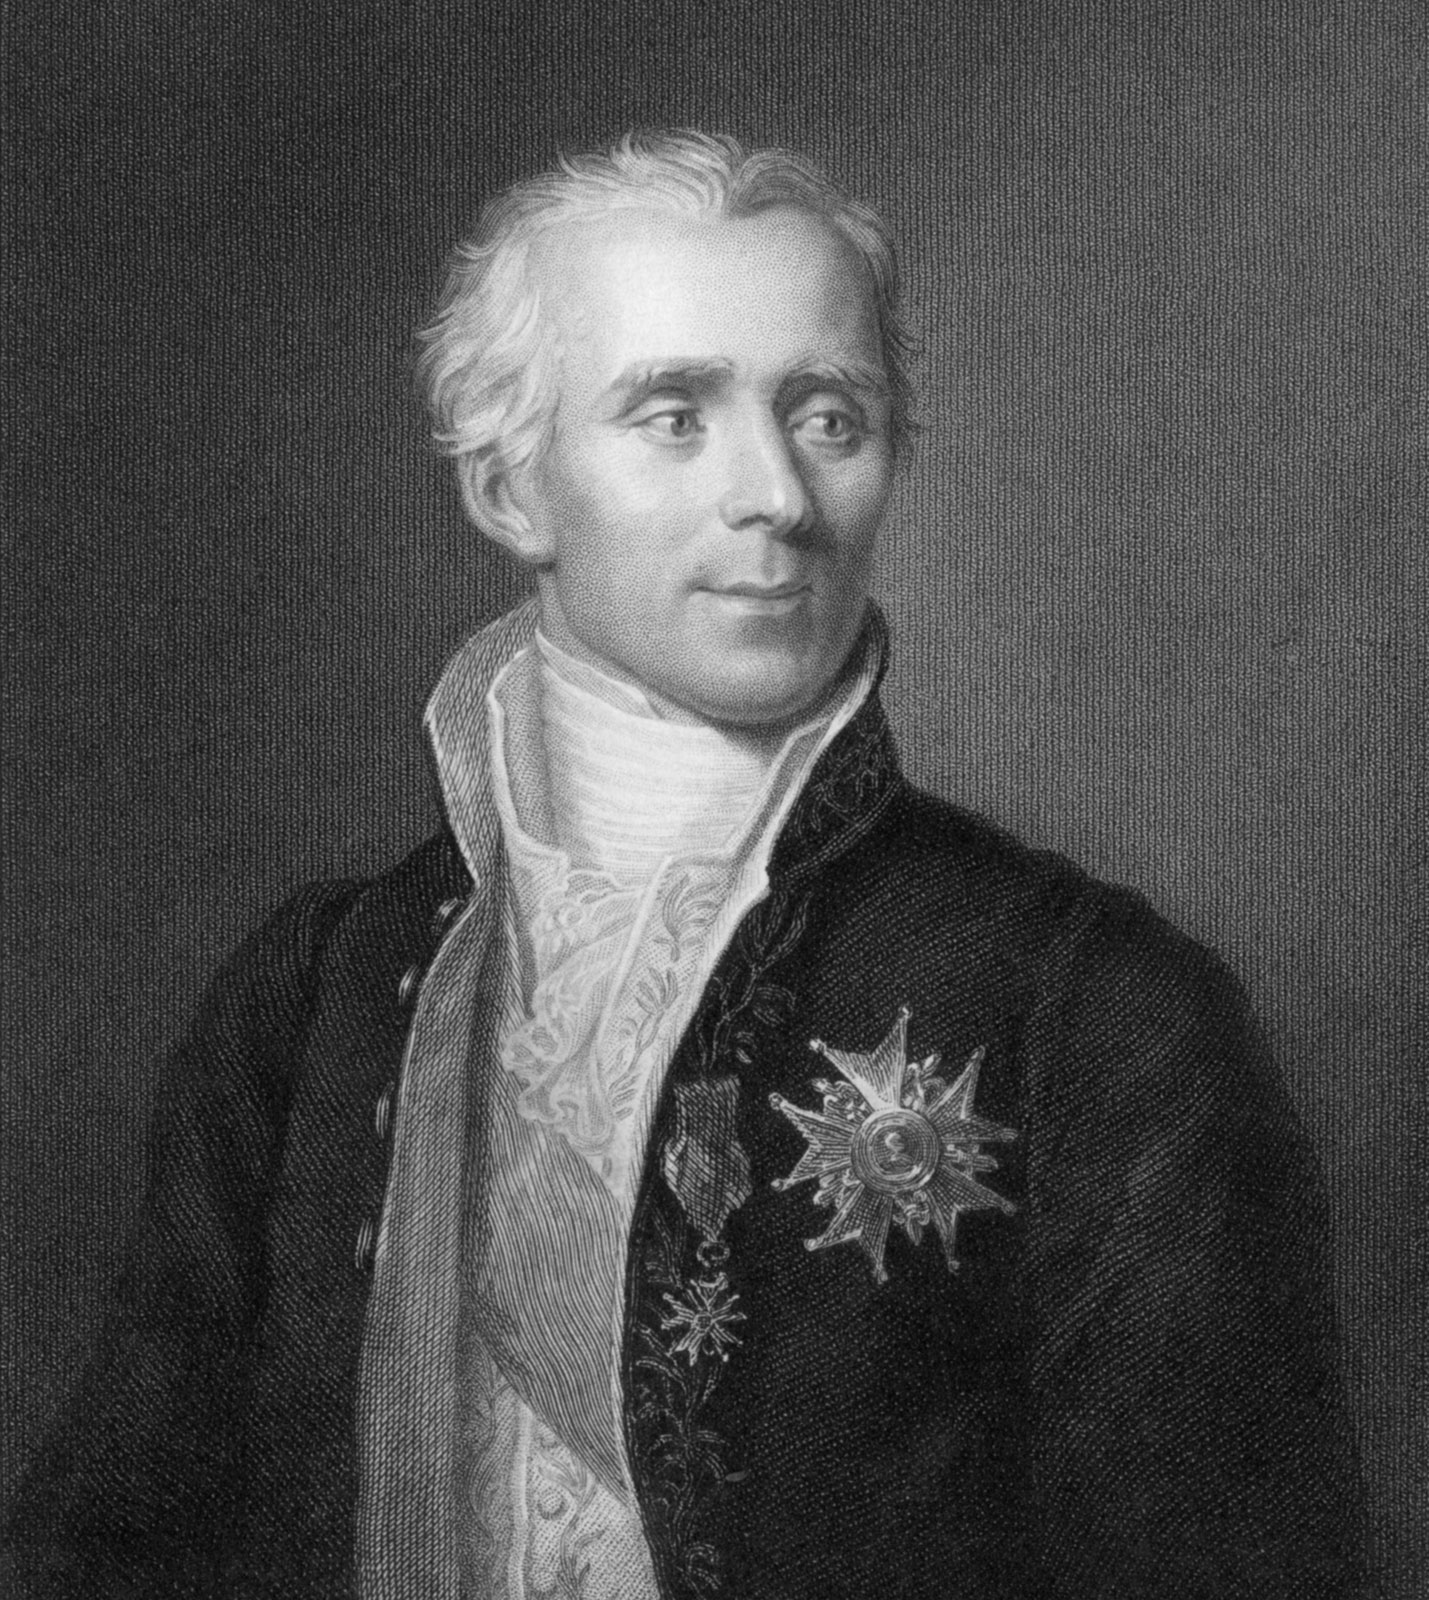
\includegraphics[width=0.8\textwidth]{./animations_figures/laplace.jpg}}
	\end{figure}
	
\end{frame}

\begin{frame}
	\frametitle{Frequentist inversion: null hypothesis testing}
	\onslide<2-> Frequentist inference considers a single hypothesis $\theta$ about data generating process at a time.
	
	\begin{align}
	\onslide<3-> {H_0&: \text{A hypothesis $\theta$ is true}}\\
	\onslide<4-> {H_1&: \text{A hypothesis $\theta$ is false}}
	\end{align}
	
	\onslide<5-> Frequentists use a rule of thumb:
	\begin{itemize}
		\item<6-> If $Pr(\text{data as or more extreme than }X|\theta) < 0.05$, then $\theta$ is false, $\implies p(\theta|X)=0$ 
		\item<7-> If $Pr(\text{data as or more extreme than }X|\theta) \geq 0.05$, then $\theta$ \textit{could} be true, $\implies p(\theta|X)=?$
	\end{itemize}
	
\end{frame}

\begin{frame}
	\frametitle{Frequentist inversion: null hypothesis testing}
	
	\begin{itemize}
		\item<2-> For $X=3$ we can carry out a series of these hypothesis tests across a range of $\theta$.
		\item<3-> For example, assume $H_0: \theta=0.5$:
	\end{itemize}
	
	\begin{figure}[ht]
		\centerline{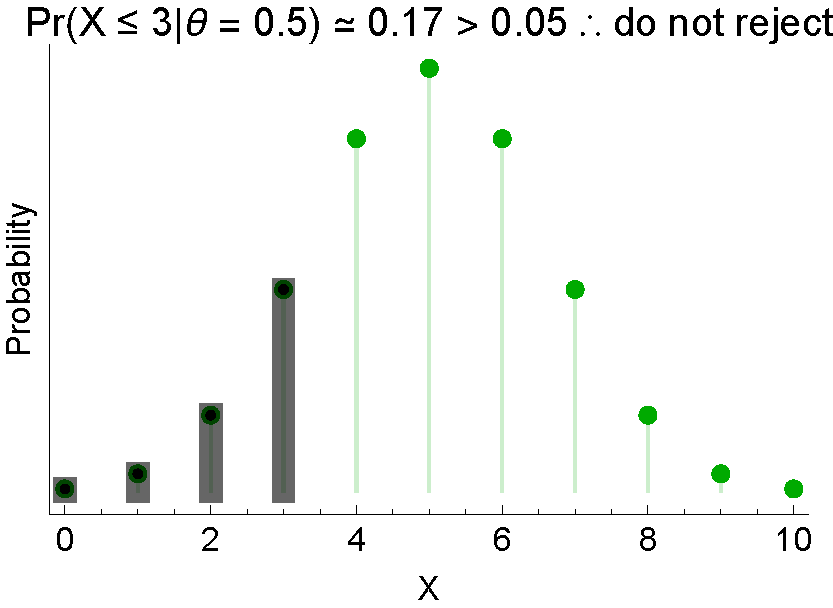
\includegraphics[width=0.8\textwidth]{animations_figures/binomial_h0_accept.pdf}}
	\end{figure}
	
\end{frame}

\begin{frame}
	\frametitle{Frequentist inversion: null hypothesis testing}
	
	\begin{itemize}
		\item<3-> Now, assume $H_0: \theta=0.8$:
	\end{itemize}
	
	\begin{figure}[ht]
		\centerline{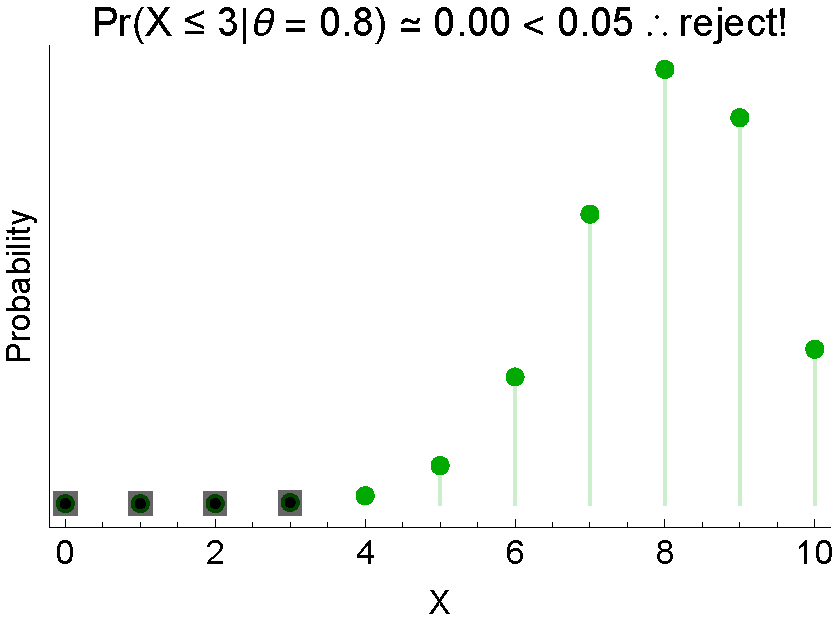
\includegraphics[width=0.8\textwidth]{animations_figures/binomial_h0_reject.pdf}}
	\end{figure}
	
\end{frame}

\begin{frame}
	\frametitle{Frequentist inversion: null hypothesis testing}
		If we carry out a series of similar hypothesis tests over the range of $\theta$ we find the 90\% confidence intervals (90\% because we have used two one sided 5\% test sizes):
		 
			\begin{equation}
			0.09 \leq \theta \leq 0.61
			\end{equation}
	
\end{frame}

\begin{frame}
	\frametitle{Bayesian inversion}
	Bayesians instead use a rule consistent with the rules of probability known as \textit{Bayes' rule}:
	
	\onslide<3->
	\begin{equation}
	p(\theta|X) = \frac{p(X|\theta)\times p(\theta)}{p(X)}
	\end{equation}
	
	Resulting in an accumulation of evidence (not binary decision) across \textit{all} potential hypotheses $\theta$.
	
\end{frame}

\begin{frame}
	\frametitle{Bayesian inversion}
	
		\begin{figure}[ht]
			\centerline{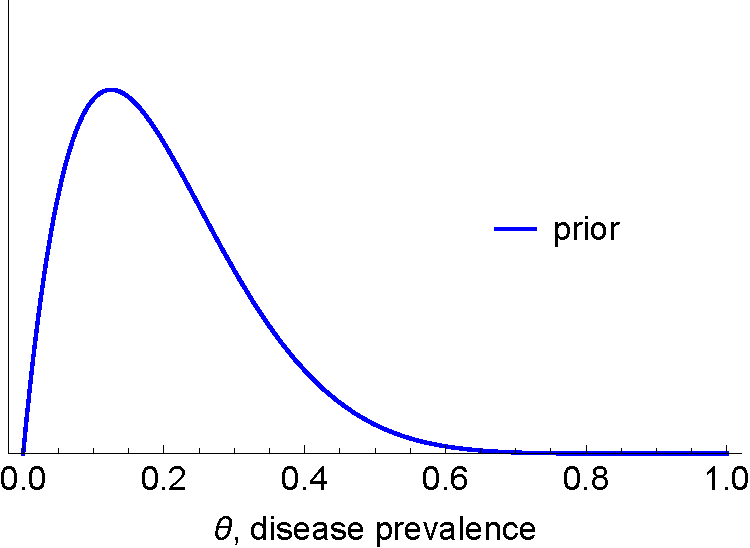
\includegraphics[width=\textwidth]{animations_figures/binomial_prior.pdf}}
		\end{figure}
	
\end{frame}

\begin{frame}
	\frametitle{Bayesian inversion}
	
	\begin{figure}[ht]
		\centerline{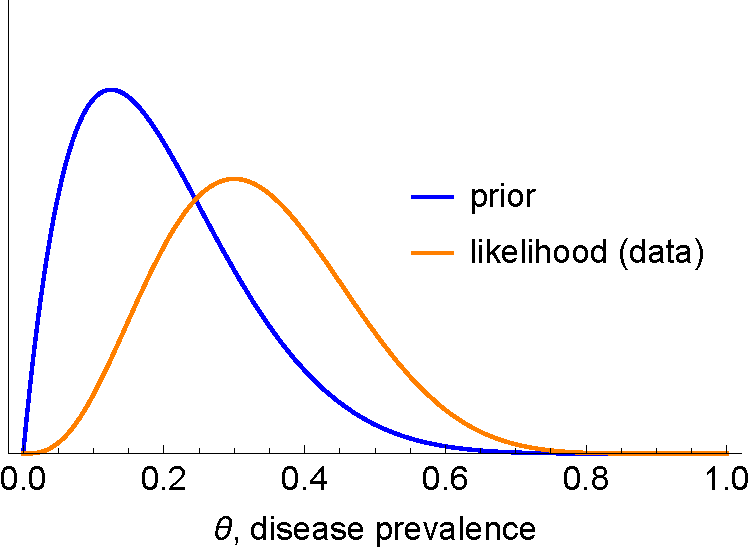
\includegraphics[width=\textwidth]{animations_figures/binomial_likelihood.pdf}}
	\end{figure}
	
\end{frame}

\begin{frame}
	\frametitle{Bayesian inversion}
	
	\begin{figure}[ht]
		\centerline{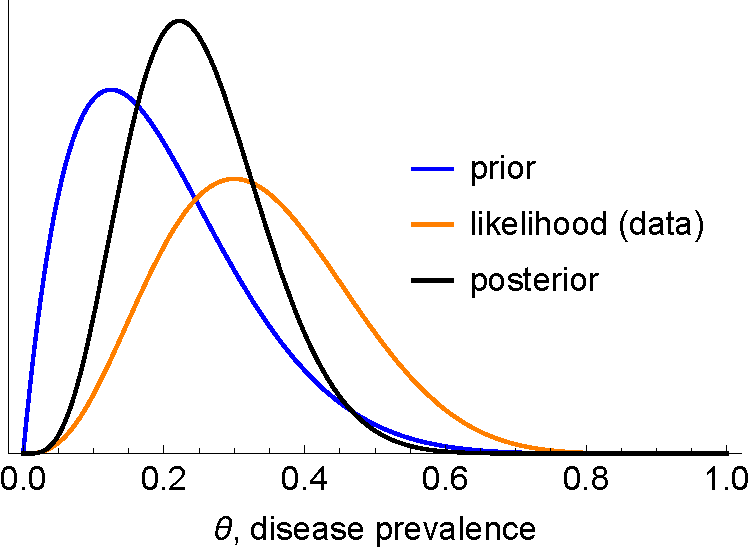
\includegraphics[width=\textwidth]{animations_figures/binomial_posterior.pdf}}
	\end{figure}
	
\end{frame}

\begin{frame}
	\frametitle{Bayesian credible intervals}
	
	\begin{figure}[ht]
		\centerline{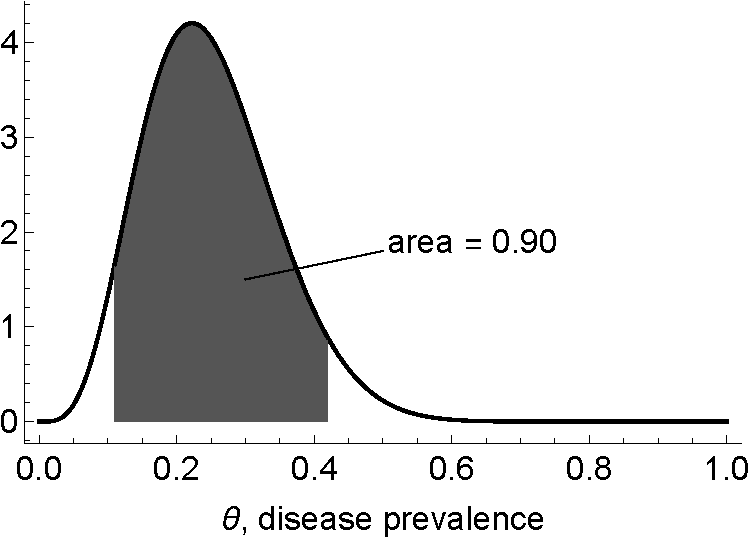
\includegraphics[width=0.75\textwidth]{animations_figures/binomial_credible_interval.pdf}}
	\end{figure}
	
	$\implies$ find a 90\% central posterior interval of $0.11\leq\theta\leq 0.41$.
	
\end{frame}

\begin{frame}
	\frametitle{}
	{\Huge Questions?}
\end{frame}

\section{Elements of Bayes' rule for inference}
\frame{\tableofcontents[currentsection]}

\begin{frame}
	\frametitle{Bayes' rule for inference}
	
	
	\begin{equation}
	p(\theta|X) = \frac{p(X|\theta)\times p(\theta)}{p(X)}
	\end{equation}
	
	But what do these terms mean?
	
\end{frame}

\begin{frame}
	\frametitle{Likelihood summary}
	
	\begin{equation}
	p(\theta|X) = \frac{\mathcircled{\color{blue}p(X|\theta)}\times p(\theta)}{p(X)}
	\end{equation}
	
	\begin{itemize}
		\item<2-> In our example, $\theta$ is the disease prevalence.
		\item<3-> $X$ is the data.
		\item<4-> $p(X|\theta)$ represents the \textit{likelihood}. 
		\item<5-> Remember \textit{not} a probability distribution because $\theta$ varies.
		\item<6-> Encapsulates many \textbf{subjective} judgements about analysis.
	\end{itemize}
	
\end{frame}

\begin{frame}
	\frametitle{Priors summary}
	\begin{equation}
	p(\theta|X) = \frac{p(X|\theta)\times \mathcircled{\color{blue}p(\theta)}}{p(X)}
	\end{equation}
	
	\begin{itemize}
		\item<2-> $p(\theta)$ represents the \textit{prior}. 
		\item<3-> A valid probability distribution.
		\item<4-> Similar to the likelihood; it is also subjective.
	\end{itemize}
\end{frame}

\begin{frame}
	\frametitle{No ``objective'' rule for priors}
	
	\begin{itemize}
		\item<2-> Embody subjective assumptions about state of the world.
		\item<3-> Essentially measure $Pr(\text{cause}|\text{pre-data knowledge})$.
		\begin{itemize}
			\item[-]<4-> Since knowledge differs between subjects $\implies$ different priors.
		\end{itemize}
		\item<5-> Can be informed by pre-experimental data (for example, previous studies or from a collection of previous studies).
	\end{itemize}
	
	\begin{figure}[ht]
		\centerline{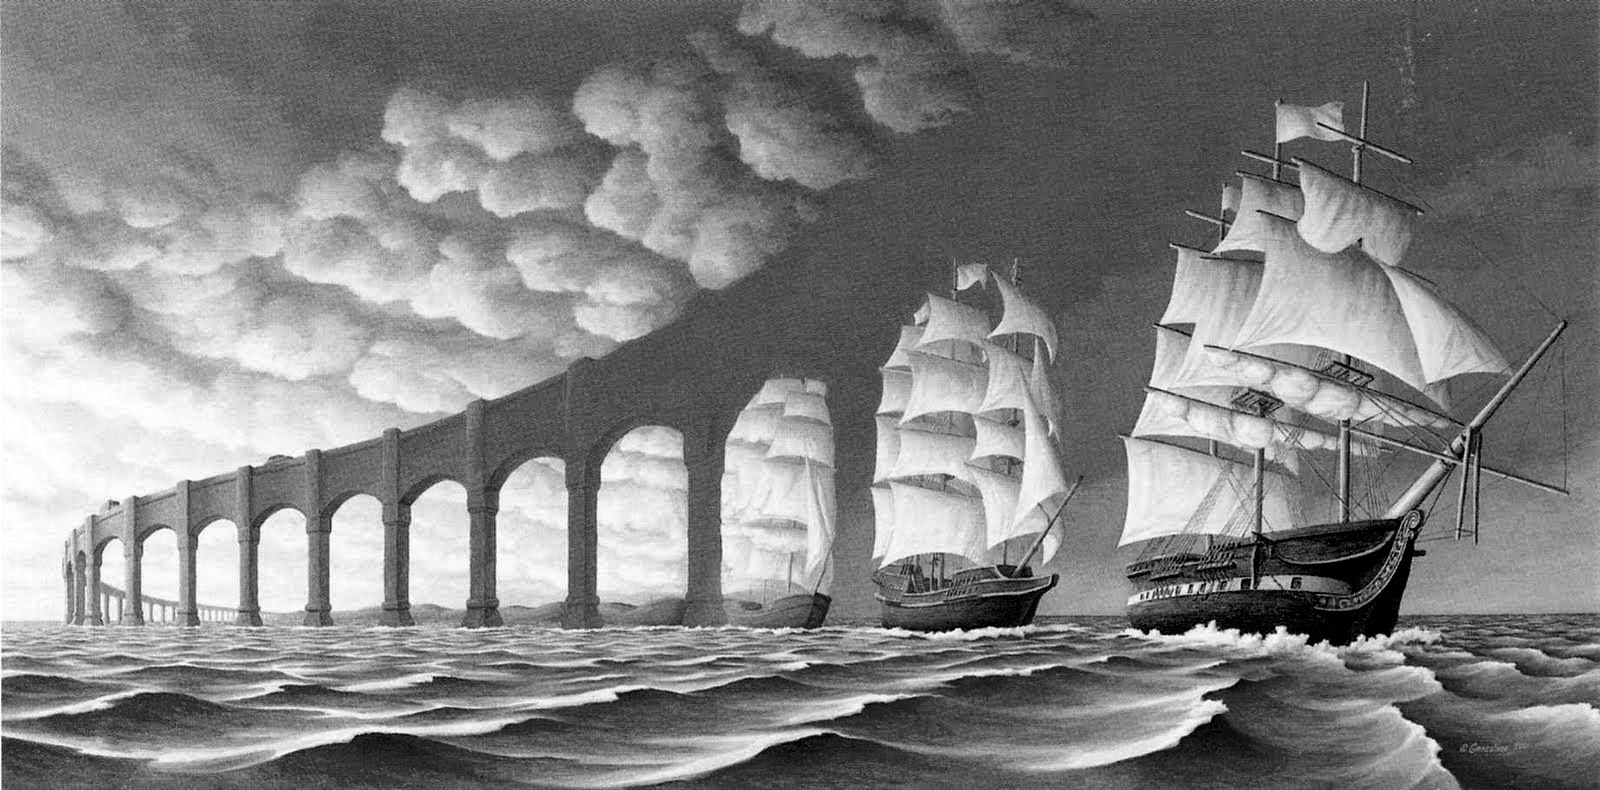
\includegraphics[width=0.8\textwidth]{./animations_figures/shipSubjective.jpg}}
	\end{figure}
	
\end{frame}

\begin{frame}
	\frametitle{Denominator summary}
	\begin{equation}
	p(\theta|X) = \frac{p(X|\theta)\times p(\theta)}{\mathcircled{\color{blue}p(X)}}
	\end{equation}
	
	\begin{itemize}
		\item<2-> $p(X)$ represents the \textit{denominator}.
		\item<3-> Two different interpretations:
		\begin{itemize}
			\item[-]<4-> Before we collect $X$ it is the \textbf{prior predictive distribution}.
			\item[-]<5-> When we have data $X=3$ it is simply a number (that normalises the posterior) known as the \textbf{evidence} or \textbf{marginal likelihood}.
		\end{itemize}
		\item<6-> Calculated from the numerator.
		\item<7-> Source of some difficulty of \textbf{exact} Bayesian inference (return to this later).
	\end{itemize}
\end{frame}

\begin{frame}
	\frametitle{Posteriors summary}
	\begin{equation}
	\mathcircled{\color{blue}p(\theta|X)} = \frac{p(X|\theta)\times p(\theta)}{p(X)}
	\end{equation}
	
	\begin{itemize}
		\item<2-> $p(\theta|X)$ represents the \textit{posterior}. 
		\item<3-> A valid probability distribution.
		\item<4-> Starting point for all further analysis in Bayesian inference.
	\end{itemize}
	
\end{frame}

\begin{frame}
	\frametitle{Intuition behind Bayesian analyses}
	\onslide<2-> Bayes' rule:
	
	\onslide<3->
	\begin{equation}
	p(\theta|X) = \frac{p(X|\theta)\times p(\theta)}{p(X)}
	\end{equation}
	
	\onslide<4-> Tells us that:
	
	\onslide<5->
	\begin{equation}
	p(\theta|X) \propto p(X|\theta)\times p(\theta)
	\end{equation}
	
	\onslide<6-> Because $p(X)$ is independent of $\theta$
	
	\onslide<7->
	$\implies$ the posterior is essentially a weighted (geometric) mean of the prior and likelihood.
	
\end{frame}

\begin{frame}
	\frametitle{Intuition behind Bayesian analyses: prior}
	Consider $N=10$ where $X=3$.
	
	\begin{figure}[t]
		\centerline{\animategraphics[width=1\textwidth,controls,buttonsize=1em,buttonfg=0.5]{2}{animations_figures/binomial_prior_}{1}{37}}
	\end{figure}
\end{frame}

\begin{frame}
	\frametitle{Intuition behind Bayesian analyses: likelihood}
	\onslide<1-> Now holding prior constant and varying $X$.
	
	\begin{figure}[t]
		\centerline{\animategraphics[width=1\textwidth,controls,buttonsize=1em,buttonfg=0.5]{1}{animations_figures/binomial_likelihood_}{1}{10}}
	\end{figure}
\end{frame}

\begin{frame}
	\frametitle{Intuition behind Bayesian analyses: sample size}
	\onslide<1-> Constant prior and proportion with disease; sample size$\uparrow$.
	
	\begin{figure}[t]
		\centerline{\animategraphics[width=1\textwidth,controls,buttonsize=1em,buttonfg=0.5]{2}{animations_figures/binomial_posterior_}{1}{20}}
	\end{figure}
\end{frame}

\begin{frame}
	\frametitle{}
	{\Huge Questions?}
\end{frame}

\section{The difficulty with exact Bayesian inference}
\frame{\tableofcontents[currentsection]}

\begin{frame}
	\frametitle{The denominator revisited}
	\begin{equation}
	p(\theta|X=3) = \frac{p(X=3|\theta)\times p(\theta)}{\mathcircled{\color{blue}p(X=3)}}
	\end{equation}
	
	\onslide<2-> Where we suppose we have $X=3$ disease-positive out of a sample of 10 in our example.
	\onslide<3-> We obtain the denominator by averaging out all $\theta$ dependence. 
	\onslide<4-> This is equivalent to integrating across all $\theta$:
	
	\onslide<5->
	\begin{equation}
	p(X=3) = \int\limits_{0}^{1} p(X=3|\theta)\times p(\theta) \mathrm{d}\theta
	\end{equation}
	
	This is equivalent to working out an \textbf{area} under a curve.
	
\end{frame}

\begin{frame}
	\frametitle{The denominator as an area}
	
	\begin{figure}
		\centerline{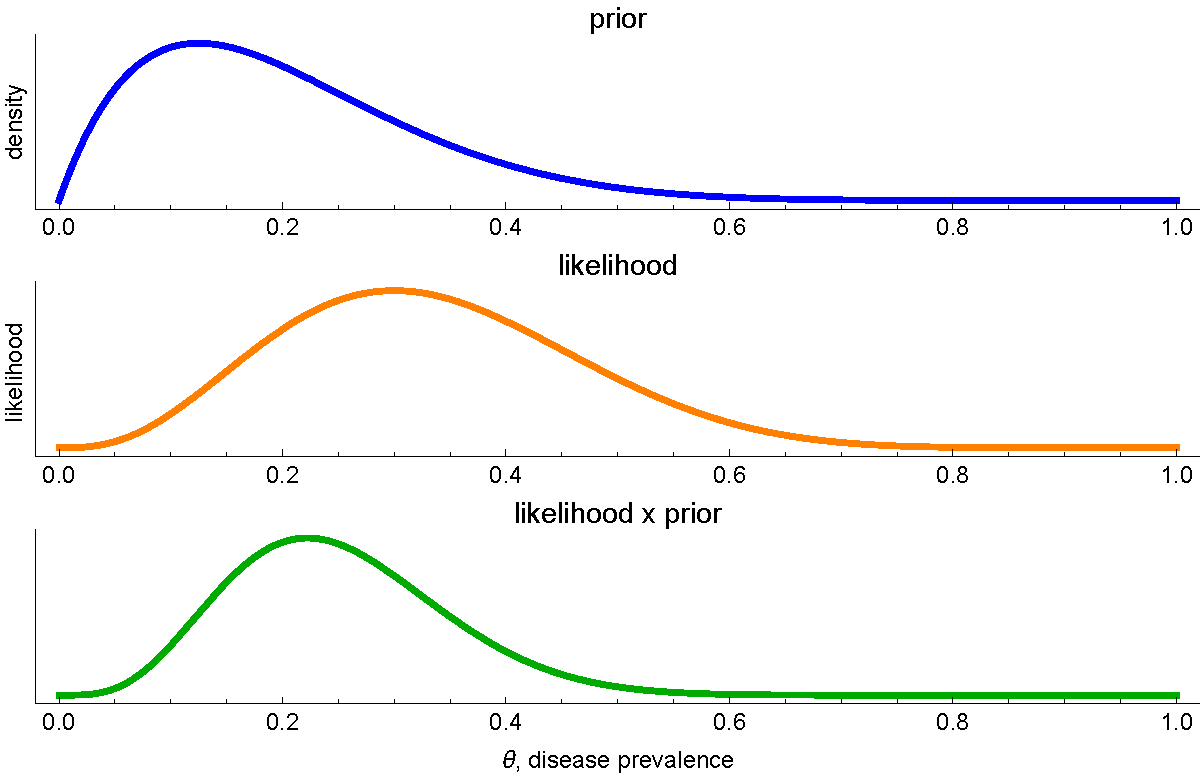
\includegraphics[width=1\textwidth]{animations_figures/binomial_area_1.pdf}}
	\end{figure}
	
\end{frame}

\begin{frame}
	\frametitle{The denominator as an area}
	
	\begin{figure}
		\centerline{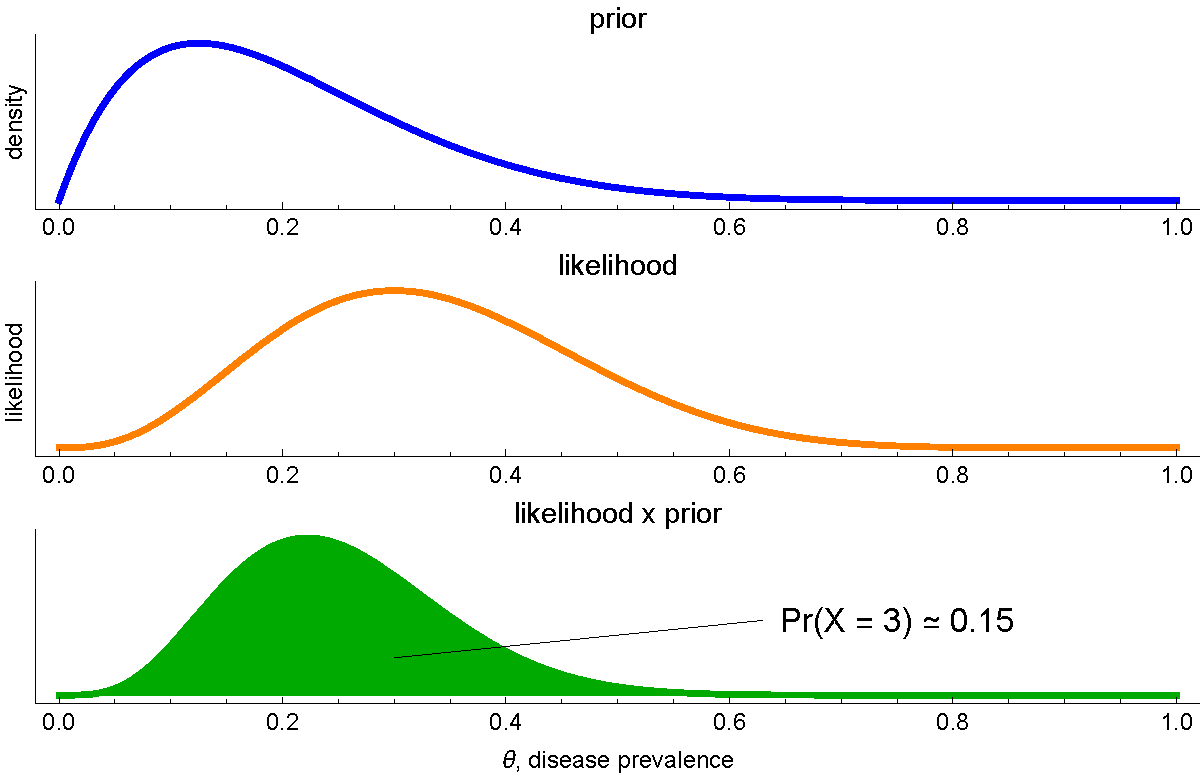
\includegraphics[width=1\textwidth]{animations_figures/binomial_area_2.pdf}}
	\end{figure}
	
\end{frame}



\begin{frame}
	\frametitle{Calculating the denominator in 2 dimensions}
	\onslide<2-> If we considered a different model where there were two parameters $\theta_1\in(0,1),\; \theta_2\in(0,1)  \implies$:
	
	\onslide<3->
	
	\begin{equation}
	p(X=3) = \int\limits_{0}^{1} \int\limits_{0}^{1} p(X=3|\theta_1,\theta_2)\times p(\theta_1,\theta_2) \mathrm{d}\theta_1 \mathrm{d}\theta_2 
	\end{equation}
	
	\onslide<4-> This is equivalent to working out a \textbf{volume} contained within a surface.
	
\end{frame}

\begin{frame}
	\frametitle{Calculating the denominator in $d$ dimensions}
	\onslide<2-> If we considered a different model where there were $d$ parameters $(\theta_1,...,\theta_d)$ all defined to lie between 0 and 1 $\implies$:
	
	\onslide<3->
	
	\begin{equation}
	p(X=3) = \int\limits_{0}^{1} ... \int\limits_{0}^{1} p(X=3|\theta_1,...,\theta_d)\times p(\theta_1,...,\theta_d) \mathrm{d}\theta_1...\mathrm{d}\theta_d
	\end{equation}
	
	\onslide<4-> This is equivalent to working out a $(d+1)$-dimensional \textbf{volume} contained within a $d$-dimensional (hyper-surface)!
	
	\onslide<5->
	\begin{figure}
		\centerline{
\includegraphics[width=0.5\textwidth]{./animations_figures/lec2_dogIroning.pdf}}
	\end{figure}
	
\end{frame}

\begin{frame}
	\frametitle{The difficult denominator}
	
	\begin{itemize}
		\item<2-> Calculating the denominator possible for $d < \sim 3$ using computers.
		\item<3-> Numerical quadrature and many other approximate schemes struggle for larger $d$.
		\item<4-> Many models have \textbf{thousands} of parameters.
	\end{itemize}
	
	\onslide<5->
	\Large Arrrghhh!
	
\end{frame}

\section{Conjugate priors}
\frame{\tableofcontents[currentsection]}

\begin{frame}
	\frametitle{What are conjugate priors?}
	
	\onslide<2->
	Judicious choice of prior and likelihood can make posterior calculation trivial.
	
	\begin{itemize}
		\item<3-> Choose a likelihood $L$.
		\item<4-> Choose a prior $\theta\sim f\in F$, where:
		\begin{itemize}
			\item[-]<5-> $F$ is a family of distributions.
			\item[-]<6-> $f$ is a member of that \textbf{same} family.
		\end{itemize}
		\item<7-> If posterior, $\theta|X\sim f'\in F$ $\implies$ conjugate!
		\item<8-> In other words both the \textbf{prior} and \textbf{posterior} are members of the same distribution!
	\end{itemize}
	
\end{frame}

\begin{frame}
	\frametitle{Conjugate priors}
	
	\begin{itemize}
		\item<3-> For likelihood (if independent and identically-distributed):
		\onslide<4-> 
		\begin{equation}
		X \sim \mathcal{B}(10,\theta)\implies p(X|\theta)\propto \theta^X (1-\theta)^{10-X}
		\end{equation}
		\item<5-> For prior assume a beta distribution (a reasonable choice if $\theta\in(0,1)$):
		\onslide<6->
		\begin{equation}
		\theta\sim \text{beta}(a,b) \implies p(\theta) \propto \theta^{a-1}(1-\theta)^{b-1}
		\end{equation}
		\item<7-> Numerator of Bayes' rule for inference: 
		\onslide<8->
		\begin{equation}
		p(X|\theta)\times p(\theta) \propto \theta^X (1-\theta)^{10-X} \times \theta^{a-1}(1-\theta)^{b-1}
		\end{equation}
	\end{itemize}
\end{frame}

\begin{frame}
	\frametitle{Conjugate priors}
	\begin{itemize}
		\item<2-> Numerator of Bayes' rule for inference: 
		\onslide<3->
		\begin{align*}
		p(X|\theta)\times p(\theta) &\propto \theta^X (1-\theta)^{10-X} \times \theta^{a-1}(1-\theta)^{b-1}\\
		\onslide<4->{&=\theta^{X+a-1} (1-\theta)^{10-X+b-1}}
		\end{align*}
		\item<5-> This has same $\theta$-dependence as a $\text{beta}(X+a,10-X+b)$ density $\implies$ must be this distribution!
		\item<6-> $\therefore$ a beta prior is \textit{conjugate} to a binomial likelihood.
	\end{itemize}
\end{frame}


\begin{frame}
	\frametitle{Table of common conjugate pairs of likelihoods and priors}
	
	\onslide<2-> {No need to do any integrals! Just lookup rules:
		
		\vspace{0.4cm}}
	
	\small
	\begin{tabular}{lll}
		\onslide<3-> \textbf{Likelihood} & \onslide<4-> \textbf{Prior} & \onslide<5-> \textbf{Posterior} \\
		\hline
		\onslide<6-> Bernoulli & \onslide<7-> $\text{beta}(\alpha,\beta)$   & \onslide<8-> $\text{beta}(\alpha+\sum\limits_{i=1}^{n}X_i,\beta+n-\sum\limits_{i=1}^{n}X_i)$ \\
		\onslide<9-> Binomial & $\text{beta}(\alpha,\beta)$  &  $\text{beta}(\alpha+\sum\limits_{i=1}^{n}X_i,\beta+\sum\limits_{i=1}^{n}N_i-\sum\limits_{i=1}^{n}X_i)$ \\
		\onslide<10-> Poisson & $\text{Gamma}(\alpha,\beta)$ &  $\text{Gamma}(\alpha+\sum\limits_{i=1}^{n}X_i,\beta+n)$\\
		\onslide<11-> Multinomial & $\text{Dirichlet}(\boldsymbol{\alpha})$ & $\text{Dirichlet}(\boldsymbol{\alpha}+\sum\limits_{i=1}^{n} \boldsymbol{X}_i)$\\
		\onslide<12-> Normal & Normal-inv-$\Gamma$ & Normal-inv-$\Gamma$ 
	\end{tabular}%
	
\end{frame}

\begin{frame}
	\frametitle{Limits of conjugate modelling}
	\onslide<2-> Using conjugate priors is limiting because:
	
	\begin{itemize}
		\item<3-> Often restricted to univariate problems.
		\begin{itemize}
			\item[-]<4-> $\implies$ we could just use numerical quadrature instead.
		\end{itemize}
		\item<5-> Required to use relevant conjugate prior for a given likelihood $\impliedby$ may not be sufficient to capture pre-data beliefs of analyst.
	\end{itemize}
	
	\onslide<1->
	\begin{figure}
		\centerline{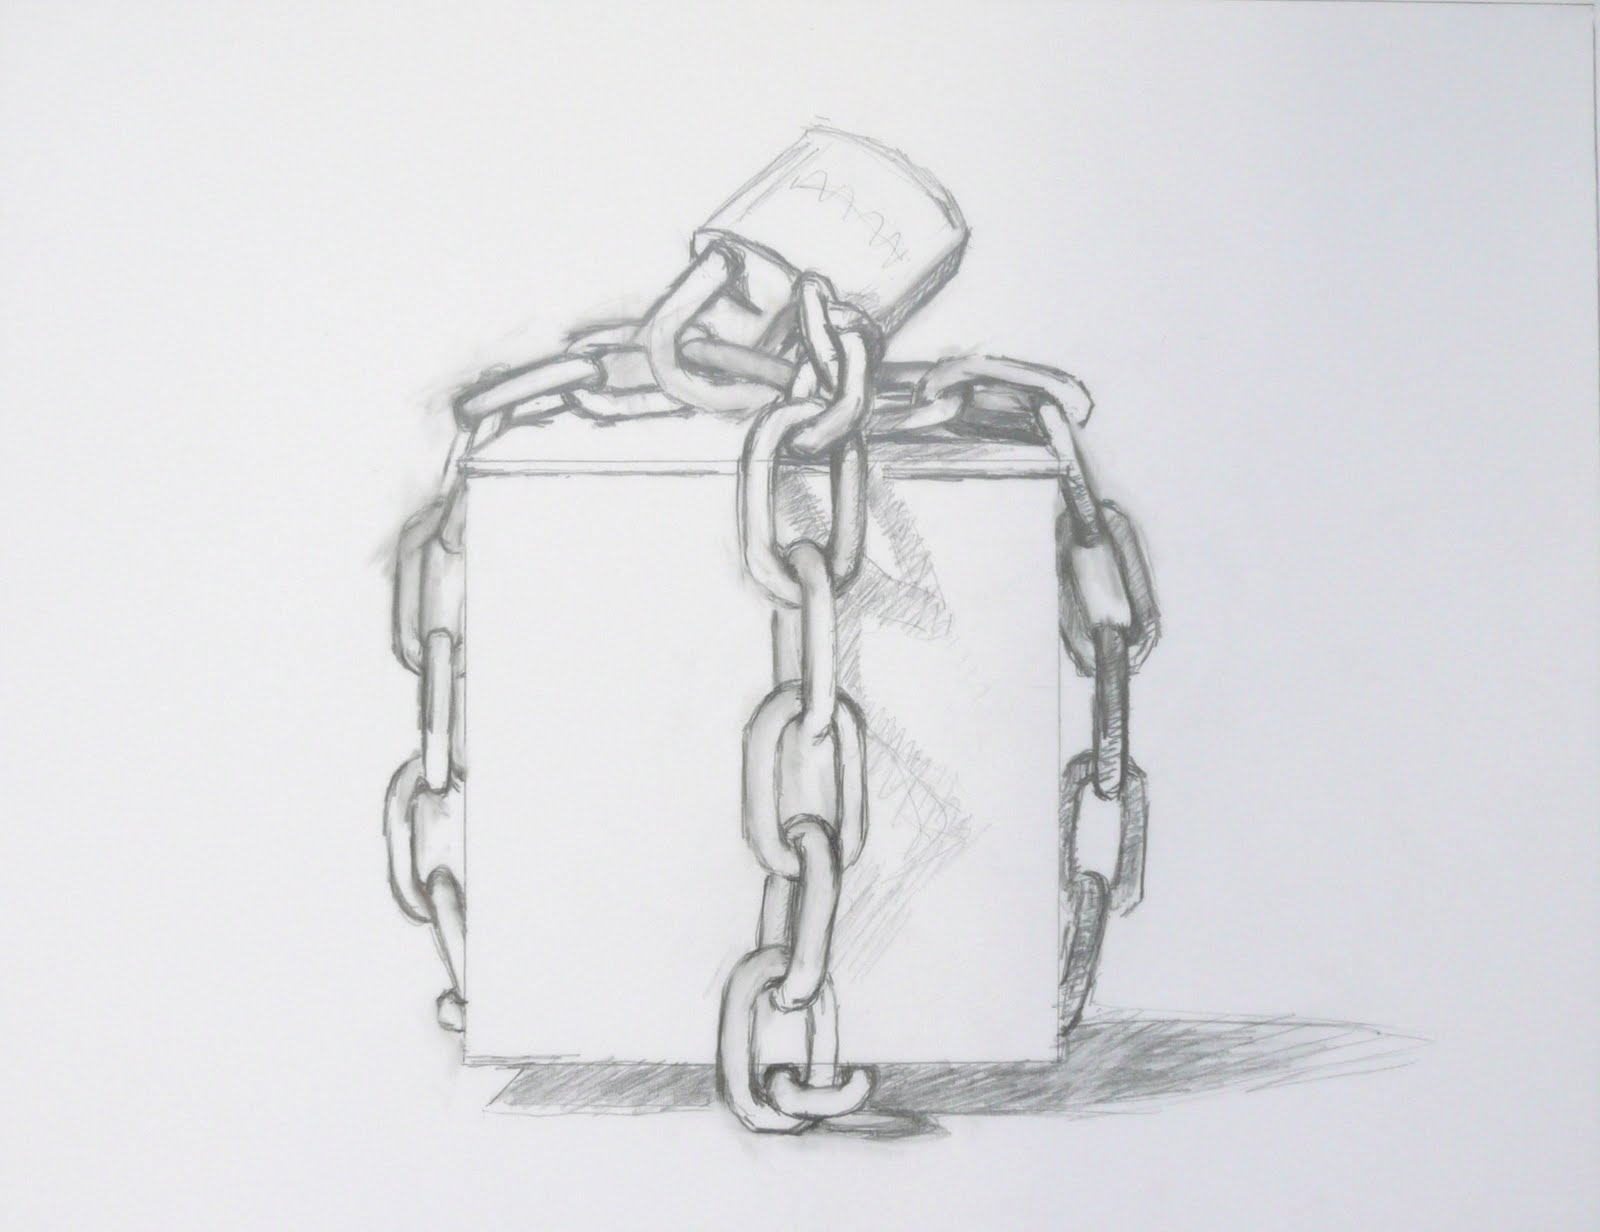
\includegraphics[width=0.7\textwidth]{./animations_figures/trapped.jpg}}
	\end{figure}
	
\end{frame}

\begin{frame}
	\frametitle{Longer-term solution}
	
	\Large Sampling (usually MCMC)! Covered this afternoon.
\end{frame}

\begin{frame}
	\frametitle{}
	{\Huge Questions?}
\end{frame}

\begin{frame}
	\frametitle{Free lectures}
	
	\begin{itemize}
		\item Richard McElreath's has a great YouTube lecture series.
		\item I have a series on YouTube called ``A Student's Guide to Bayesian Statistics''.
	\end{itemize}
	
\end{frame}


\begin{frame}
	\frametitle{Not sure I understand?}
	
	\onslide<1-> Bayesian statistics:{
		\begin{equation}
		p(\theta|\boldsymbol{D}) = \frac{p(\boldsymbol{D}|\theta)\times p(\theta)}{p(\boldsymbol{D})}
		\end{equation}}
	
	\onslide<1-> Beigeian statistics:{
		\begin{equation}
		\textcolor{beige}{p(\theta|\boldsymbol{D}) = \frac{p(\boldsymbol{D}|\theta)\times p(\theta)}{p(\boldsymbol{D})}}
		\end{equation}}
	
\end{frame}

\end{document}
